%% Calibration deck: columns [t] and [T] below a paragraph, a list beside a figure, a table.
\setSlideVersion{1-0-0}
\begin{standardframe}{Columns, a paragraph above, and a table}
	{\small A paragraph first, so the columns below it do not start the frame.\par}
	\medskip
	\begin{columns}[t,onlytextwidth]
		\begin{column}{0.46\linewidth}
			\begin{itemize}
				\item A list in a top-aligned column
				\item Second item
			\end{itemize}
		\end{column}
		\begin{column}{0.46\linewidth}
			\begin{itemize}
				\item The same, beside it
				\item Second item
			\end{itemize}
		\end{column}
	\end{columns}
	\medskip
	\begin{columns}[T,onlytextwidth]
		\begin{column}{0.46\linewidth}
			\begin{SMTable}[gap=12pt]{lcc}
				\toprule
				Frame & Title bar & Footer \\
				\midrule
				\SMCode{standardframe} & yes & yes \\
				\SMCmd{fullbleedframe} & no & no \\
				\bottomrule
			\end{SMTable}
		\end{column}
		\begin{column}{0.46\linewidth}
			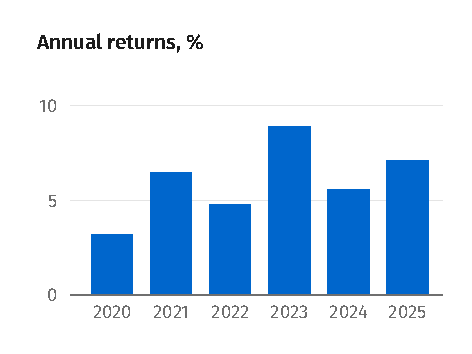
\includegraphics[height=2cm]{media/illustration-bar-chart.pdf}
		\end{column}
	\end{columns}
\end{standardframe}
